\documentclass[]{article}
\usepackage{hyperref}
\usepackage{caption}
\usepackage{graphicx}
\graphicspath{{../signatures/}}

% Imported Packages
%------------------------------------------------------------------------------
\usepackage{amssymb}
\usepackage{amstext}
\usepackage{amsthm}
\usepackage{amsmath}
\usepackage{enumerate}
\usepackage{float}
\usepackage{fancyhdr}
\usepackage[margin=1in]{geometry}
\usepackage{graphicx}
%\usepackage{extarrows}
%\usepackage{setspace}
%\usepackage{xcolor}
\usepackage{color}
\usepackage{multirow}
%------------------------------------------------------------------------------

% Header and Footer
%------------------------------------------------------------------------------
\pagestyle{plain}  
\renewcommand\headrulewidth{0.4pt}                                      
\renewcommand\footrulewidth{0.4pt}                                    
%------------------------------------------------------------------------------

% Title Details
%------------------------------------------------------------------------------
\title{Deliverable \#1 Template : Software Requirement Specification (SRS)}
\author{SE 3A04: Software Design II -- Large System Design}
\date{18 February 2024}
                            
%------------------------------------------------------------------------------

% Document
%------------------------------------------------------------------------------
\begin{document}

\maketitle
\noindent{\bf Tutorial Number:} T01\\
{\bf Group Number:} G07 \\
{\bf Group Members:}
\begin{itemize}
	\item Awurama Nyarko
	\item Chelsea Maramot
	\item Harrison Chiu
	\item Khushi Bhojane
	\item Sumanya Gulati
\end{itemize}

\newpage
\section{Introduction}
\label{sec:introduction}
% Begin Section
This Software Requirements Specification (SRS) will outline the requirements and guidelines for the development of SecureChat. SecureChat is a secure communication application designed specifically for the purpose of organizational usage. This document will be discussing the applications purpose, scope, user characteristics, and an overview of the product’s overall functionalities. SecureChat will be employing robust cryptographic measures, as well as secure authentication protocols to protect sensitive information/ data and ensure secure internal communications.

\subsection{Purpose}
\label{sub:purpose}
% Begin SubSection
This SRS focuses on functional requirements, non-functional requirements, user interactions, and security protocols for the SecureChat application.\\
\newline
This document is written for the intention of usage by a broad audience including project managers, software developers, security analysts, and stakeholders. No prerequisite knowledge or readings is expected or required.
% End SubSection

\subsection{Scope}
\label{sub:scope}
% Begin SubSection
The SecureChat application is the primary software product to be developed. It is designed as an encrypted messaging app for deployment on company-issued Android devices.\\
\newline
SecureChat will integrate a Key Distribution Centre (KDC) to manage cryptographic keys and employ an authentication protocol to validate user identities. It will utilize symmetric-key encryption to ensure secure communications within the app. The application is designed to facilitate secure text messaging, file sharing, and guarantee the integrity and confidentiality of chat logs. Additional functionalities include dynamic key generation and rotation, enhancing the app's resilience against potential security threats.\\
\newline
The objective of SecureChat is to establish a secure, efficient communication channel within an organization, mitigating risks associated with corporate espionage. By utilizing advanced cryptographic techniques, SecureChat aims to protect sensitive information while maintaining user-friendly operations. Additionally, it seeks to foster trust among employees regarding the organization's commitment to security and privacy. Through these measures, SecureChat aims to offer a robust solution for secure internal communications, thereby protecting against data breaches and unauthorized access to sensitive information.
% End SubSection

\subsection{Definitions, Acronyms, and Abbreviations}
\label{sub:definitions_acronyms_and_abbreviations}
% Begin SubSection
\begin{itemize}
	\item \textbf{KDC (Key Distribution Center):} A central authority in cryptographic systems that is responsible for distributing secret keys to parties wishing to communicate securely.
	\item \textbf{Multimedia Files:} Digital files that incorporate content in multiple forms such as text, audio, images, animations, video, and interactive content.
	\item \textbf{PIPEDA (Personal Information Protection and Electronic Documents Act):} A Canadian federal privacy law regulating the collection, use, and disclosure of personal information in the course of commercial activities.
	\item \textbf{WCAG (Web Content Accessibility Guidelines):} A set of guidelines developed through the W3C process, aimed at making web content more accessible to people with disabilities.
\end{itemize}
% End SubSection

\subsection{References}
\label{sub:references}
% Begin SubSection
	\begin{thebibliography}{99}
		\bibitem{1c} “5 Ultimate Steps To Customize Your Windows Folders to Increase Productivity.” Accessed: Feb. 17, 2024. [Online]. Available: \url{https://www.linkedin.com/pulse/5-ultimate-steps-customize-your-windows-folders-increase-do/}

		\bibitem{2c} “Web Content Accessibility Guidelines (WCAG) 2.1.” Accessed: Feb. 17, 2024. [Online]. Available: \url{https://www.w3.org/TR/WCAG21/}

		\bibitem{3c} “How To Set Up Optimal Chat for Your Real-Time Application.” Accessed: Feb. 17, 2024. [Online]. Available: \url{https://subspace.com/resources/optimal-chat-real-time}

		\bibitem{4c} N. Mansour, “Mobile App Quality: An Essential Guide | Instabug.” Accessed: Feb. 17, 2024. [Online]. Available: \url{https://www.instabug.com/blog/mobile-app-quality-an-essential-guide}

		\bibitem{5c} “8 Ways to Effectively Reduce Server Response Time,” DataDome. Accessed: Feb. 17, 2024. [Online]. Available: \url{https://datadome.co/learning-center/how-to-reduce-server-response-time/}

		\bibitem{6c} SentinelOne, “SentinelOne | Service Availability: What It Is and Metrics You Should Know,” SentinelOne. Accessed: Feb. 17, 2024. [Online]. Available: \url{https://www.sentinelone.com/blog/service-availability-and-metrics/}

		\bibitem{7c} “Our Experience with Modular Architecture,” TRIARE. Accessed: Feb. 17, 2024. [Online]. Available: \url{https://triare.net/insights/modular-architecture-2/}

		\bibitem{8c} kavinrajan, “Suggested Minimum Android version 2021,” Medium. Accessed: Feb. 17, 2024. [Online]. Available: \url{https://medium.com/@kavinece53/suggested-minimum-android-version-2021-affba3ef74f}

		\bibitem{9c} “Google Play.” Accessed: Feb. 17, 2024. [Online]. Available: \url{https://play.google.com/about/developer-distribution-agreement.html}

		\bibitem{10c} O. of the P. C. of Canada, “PIPEDA fair information principles.” Accessed: Feb. 17, 2024. [Online]. Available: \url{https://www.priv.gc.ca/en/privacy-topics/privacy-laws-in-canada/the-personal-information-protection-and-electronic-documents-act-pipeda/p_principle/}

		\bibitem{11c} “Core app quality,” Android Developers. Accessed: Feb. 17, 2024. [Online]. Available: \url{https://developer.android.com/docs/quality-guidelines/core-app-quality}
	\end{thebibliography}
% End SubSection


\subsection{Overview}
\label{sub:overview}
% Begin SubSection
Following this introduction, Section 2 provides an in-depth description of the product, outlining its perspective, functionalities, and the general factors influencing its design and requirements. Section 3 presents the Use Case Diagram, offering a visual representation of the system's operational scenarios. Section 4 will go into the Highlights of Functional Requirements, detailing the actions and processes SecureChat is designed to perform. Categorizing them with business events and viewpoints. Section 5 will detail the Non-Functional Requirements, including the system's performance, usability, and security standards. Comprehensively these sections construct a framework for the development of SecureChat, ensuring there is clarity and a sense of direction throughout the project lifecycle.
% End SubSection

% End Section

\section{Overall Product Description}
\label{sec:overall_description}
% Begin Section

\subsection{Product Perspective}
\label{sub:product_perspective}
% Begin SubSection
SecureChat is a chat-based application developed for a specific organization and its employees. Similar, commerically available tools incude popular workplace collaboration softwares like Slack, Microsoft Teams and Discord as well as popular instant messaging services such as WhatsApp, Facebook Messenger and Telegram. SecureChat is designed to be an amalgamation of both of these services and provide secure communication channels for its users.\\
\newline
The app allows users to communicate using individual user-to-user chats or group chats involving multiple users (with a maximum limit of 50). To allow for seamless communication, SecureChat has file sharing functionality that allows users to modify file permissions and share them securely in individual or group chats. Although, user profiles can only be created or deleted by administration for security measures, users are able to modify their personal details as well as details and permissions for group chats (such as name, description and more). Most of these features can be found in the workplace collaboration softwares and instant messaging services listed above.\\
\newline
The product is a standalone application that is expected to be a part of the organization's existing IT infrastructure. In term of security measures, the app interacts with a KDC server that generates and sends all keys to users at the starting of all secure communication sessions. For regulatory and compliance concerns, the chat history logs for all communication sessions including details such as user profiles, time stamps and message content are securely stored on a server for 2 years from the original timestamp.\\
\newline
\begin{figure}[H]
	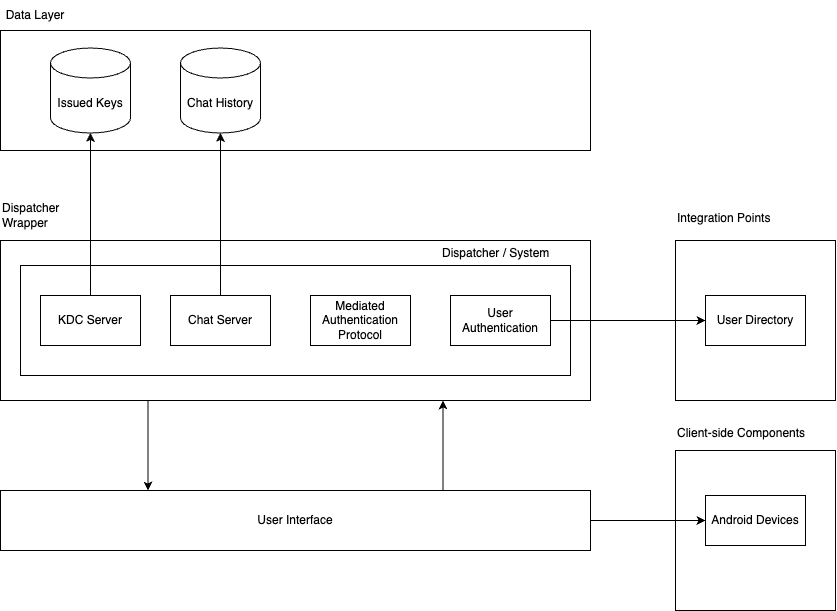
\includegraphics[scale=0.5]{system-diagram.png}
	\caption{System Diagram}
\end{figure}
% End SubSection

\subsection{Product Functions}
\label{sub:product_functions}
% Begin SubSection
A list of the modules of the product and their major functions has been provided below:

% Please add the following required packages to your document preamble:
% \usepackage{graphicx}
\begin{table}[]
\resizebox{\textwidth}{!}{%
\begin{tabular}{|l|l|}
\hline
\multicolumn{1}{|c|}{\textbf{Modules}} & \multicolumn{1}{c|}{\textbf{Functions}}                                                                                                                                                                                                                                                                                                                                                                                                                                                                                                                                                                                                                                                                                                         \\ \hline
Account and User Profile Service       & \begin{tabular}[c]{@{}l@{}}1. Login\\ - Allows user to login or logout of their account using their employee credentials.\\ 2. Update User Profile\\ - Allows user to modify their profile and status.\end{tabular}                                                                                                                                                                                                                                                                                                                                                                                                                                                                                                                             \\ \hline
Chats Service                          & \begin{tabular}[c]{@{}l@{}}1. Create Chat\\ - Allows user to start an  individual chat with another user or create a new group chat.\\ - Allows user to send and receive text messages or share files.\\ 2. Modify Group Chat\\ - Allows user to set permissions or modify details of a group chat.\\ - Allows user to add new members to a group chat or remove existing members from a group chat.\\ 3. Receive Notifications\\ - Allows user to be notified whenever a new message is received in a chat or when group chat details are modified.\\ 4. Modify Messages\\ - Allows user to modify messages after they have been sent.\\ 5. Unsend Messages\\ - Allows user to unsend a message in a chat after it has been sent.\end{tabular} \\ \hline
Security Service                       & \begin{tabular}[c]{@{}l@{}}1. Issue Keys\\ - The KDC server issues keys and sends them to communicating agents.\end{tabular}                                                                                                                                                                                                                                                                                                                                                                                                                                                                                                                                                                                                                    \\ \hline
\end{tabular}%
}
\end{table}

\begin{figure}[H]
	\centering
	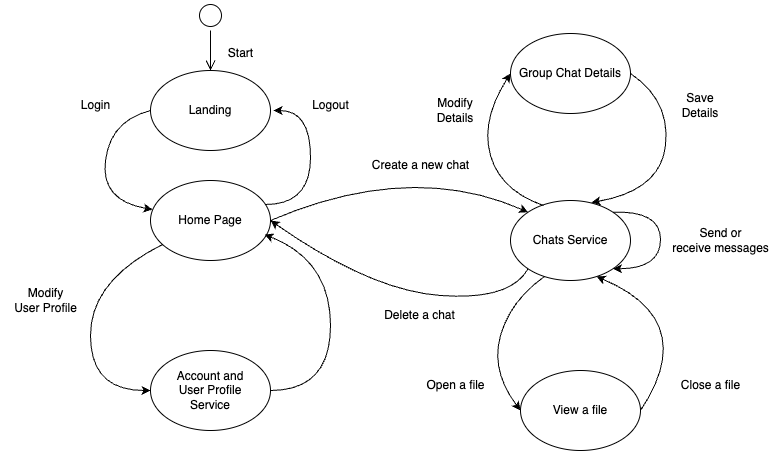
\includegraphics[scale=0.6]{state-diagram.png}
	\caption{State Diagram}
\end{figure}
% End SubSection


\subsection{User Characteristics}
\label{sub:user_characteristics}
% Begin SubSection
SecureChat is intended to be a user-friendly app designed for the current employees of a specific organization. As a result, the following are the minimum qualifications expected from all users:
\begin{itemize}
	\item \textbf{Education Level:} Basic literacy skills
 	\begin{itemize}
  		\item Users are expected to possess basic English literacy skills, specifically reading and writing.
    		\item The interface of the app is intended to be intuitive and user-friendly with clear instructions provided for using security features. This means that users with varying levels of education should be able to use the app.
      	\end{itemize}
 	\item \textbf{Technical Expertise:} Basic smartphone navigation skills
  	\begin{itemize}
   		\item Users are expected to have basic smartphone (specifically, Android) navigation skills.
     		\item Although not mandatory, ideally, users should have basic security awareness about concepts such as password security, phishing awareness, data encryption and more.
       	\end{itemize}
  	\item \textbf{Experience:} Familiarity with chat-based services
   	\begin{itemize}
    		\item Users are expected to possess prior experience using commonly used communication tools and technologies. This can include familiarity with instant messaging apps, email services or collaboration platforms such as Microsoft Teams, Slack, Discord etc.
      	\end{itemize}
   	\item \textbf{Security Clearance:} Currently employed by the organization
    	\begin{itemize}
     		\item Users must be currently employed by the organization and be permitted to use the application.
       		\item Users are expected to possess an Android device issued by the organization.
	\end{itemize}
\end{itemize}
% End SubSection

\subsection{Constraints}
\label{sub:constraints}
% Begin SubSection
\begin{itemize}
	\item \emph{Budget}: The allocated budget of the project will directly impact the technologies developers can use as well as the features that can be included in the initial launch of the application. As of the latest update to this SRS document, the budget allocated to the project is 0 CAD.
 	\item \emph{Project Timeline}: Time allocated to the development of the application will affect the scale of the project and the scope of features deployed.
  	\item \emph{Regulatory Compliance}: The application must adhere to relevant regulatory requirements including but not limited to, PIPEDA and industry-specific data storage guidelines for periodic audits.
   	\item \emph{Compatibility Requirements}: The application must be compatible with the organization's existing IT infrastructure and network configurations. Additionally, it must compatible with Android devices.
\end{itemize}
% End SubSection

\subsection{Assumptions and Dependencies}
\label{sub:assumptions_and_dependencies}
% Begin SubSection
\begin{itemize}
	\item It is assumed that the app can only be used by current employees and that a user's access to the app must be revoked when and if they leave the organization.
 	\item It is assumed that all users of the app have access to Android devices issued by the organization.
  	\item It is assumed that users will have reliable internet connectivity at all times while using the application. Currently, offline capabilities for users with limited or intermittent internet access is not implemented.	
   	\item It is assumed that the app is used only by employees who reside in Canada. Usage of the app outside of the country is assumed to be restricted.
    	\item It is assumed that all user profiles must be created/deleted and approved by the administration. Users cannot create new profiles or delete existing profiles on their own.
    	\item Innovative feature: Users are allowed to send disappearing messages for as an enhanced security measure. 
\end{itemize}
Other dependencies that directly impact the app and in case of failure could require a change to the requirements include:
\begin{itemize}
	\item The app must be compatible with the latest available version of Android.
 	\item Since the functionality of the app relies on the availability and proper functioning of a KDC server, any downtime or unexpected disruptions to the server could impact the user's ability to authenticate and securely communicate using the application.
\end{itemize}
% End SubSection

\subsection{Apportioning of Requirements}
\label{sub:apportioning_of_requirements}
% Begin SubSection
\begin{itemize}
	\item Integration with third-party services
 	\begin{itemize}
  		\item The app can have possible integrations with third-party services like email services, video conferencing platforms and more.
    	\end{itemize}
     	\item Offline mode
      	\begin{itemize}
  		\item Currently, the app relies on internet connectivity for receiving keys from the KDC server and authenticating users for each communication session. Alternate methods for authentication that reduce dependency on internet connectivity can be explored in the future.
    	\end{itemize}
     	\item Advanced search and filtering
      	\begin{itemize}
       		\item Functionality for filtering through conversations using keywords and searching for specific files shared within a chat can be added in future versions of the application.
	\end{itemize}
  	\item Additional security measures
   	\begin{itemize}
    		\item Measures such as two-factor authentication, data loss preventation and more can be deferred to subsequent releases.
      	\end{itemize}
\end{itemize}
% End SubSection

% End Section
\section{Use Case Diagram}
\label{sec:use_case_diagram}
% Begin Section
\begin{figure}[H]
	\centering
	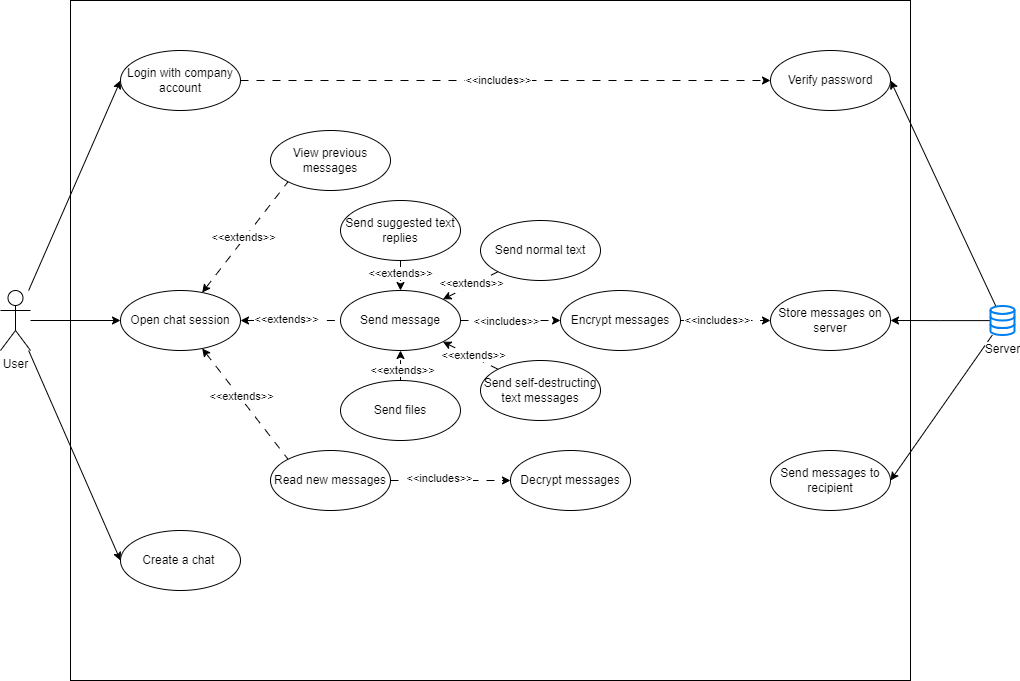
\includegraphics[width=1\textwidth]{figures/usecase.drawio.png}
	\caption{Use Case Diagram of the Project}
\end{figure}

The diagram illustrates the main usage of the application by its users, which is to communicate
with other users through file or text messages. These actions involve the server which sends the
messages to the intended recipient.

%In this section, select the most important Business Event that your system responds to and give its use case diagram.  Only one use case diagram is needed.  Give a brief textual description of the use case without repeating what is in the scenarios of the corresponding Business Event.

%
%
%
%This section should provide a use case diagram for your application. 
%\begin{enumerate}[a)]
%	\item Each use case appearing in the diagram should be accompanied by a text description. 
%\end{enumerate}
%% End Section

\section{Highlights of Functional Requirements}
\label{sec:functional_requirements}
% Begin Section


\noindent {\bf Main Business Events:} \begin{itemize}
    \item {\bf BE1: Employees}
    \item {\bf BE2: IT Support Team}
    \item {\bf BE3: Organization}
    \item {\bf BE4: Employees}
    \item {\bf BE5: IT Support Team}
    \item {\bf BE6: Organization}
    \item {\bf BE7: Employees}
    \item {\bf BE8: IT Support Team}
    \item {\bf BE9: Organization}
    \item {\bf BE10: Employees}
    \item {\bf BE11: IT Support Team}
\end{itemize}

\noindent {\bf Viewpoints:} \begin{itemize}
    \item {\bf VP1: Employees}
    \item {\bf VP2: IT Support Team}
    \item {\bf VP3: Organization}
\end{itemize}

\noindent {\bf Interpretation:} N/A

%%BUSINESS EVENT 1
	
	\begin{enumerate}[\bf {BE}1.]
		\item Authorizing an employee to use the chat application for work purposes.
		\item {\bf VP3: Organization}
			
			\noindent\fbox{%
				\parbox{1.0\textwidth}{%
					\begin{itemize}
						\item {\bf $S_{1}$:} The organization provides a list of authorized individuals to the IT Support team.
					\end{itemize}
				}%
			}
                \item {\bf VP2: IT Support Team}
			
			\noindent\fbox{%
				\parbox{1.0\textwidth}{%
					\begin{itemize}
						\item {\bf $S_{1}$:} The IT Support team grants authorization to the individuals to gain access and use the application.
					\end{itemize}
				}%
			}
%			
		
		\item[] {\bf Global Scenario of {\it Authorizing an employee to use the chat application for work purposes.}:} \newline
		\noindent\fbox{%
			\parbox{1.0\textwidth}{%
				\begin{itemize}
                        \item {\bf $S_{1}$:} The organization provides a list of authorized individuals to the IT Support team. \textcolor{green}{Proceed to E.1}.
					  \item {\bf $E_{1}$:} The IT Support team grants authorization to the individuals to gain access and use the application.\textcolor{green}{Proceed to S.2}.
					  \item {\bf $S_{2}$:} Employees now have access to the system and are authorized to use it.
                            
						
						
				\end{itemize}
			}%
		}%
		\end{enumerate}


%%BUSINESS EVENT 2
	
	\begin{enumerate}[\bf {BE}2.]
		\item Logging onto the chat application
		\item {\bf VP1: Employee}
			
			\noindent\fbox{%
				\parbox{1.0\textwidth}{%
					\begin{itemize}
						\item {\bf $S_{1}$:} System displays required login fields.
						\item {\bf $E_{1}$:} User inputs personal login information.
						\item {\bf $S_{2}$:}  Information is verified by the system. 
						\item {\bf $E_{2}$:}  User is sent a verification code. 
						
						\item {\bf $S_{3}$:}  User enters code. 
						\item {\bf $S_{(4)}$:} System reviews code and if correct, allows user access to the application.
					\end{itemize}
				}%
			}
%			
		
		\item[] {\bf Global Scenario of {\it Logging onto the chat application}:} \newline
		\noindent\fbox{%
			\parbox{1.0\textwidth}{%
				\begin{itemize}
                        \item {\bf $S_{1}$:} System displays required login fields. \textcolor{green}{Proceed to E.1}.
					  \item {\bf $E_{1}$:} User inputs personal login information.\textcolor{green}{Proceed to S.2}.
					  \item {\bf $S_{2}$:}  Information is verified by the system.
                            \begin{itemize}
                                {\bf $S_{2}.1$} The user information is inaccurate. \textcolor{red}{Loop to S.1}.
                                {\bf $S_{2}.2$} The user information is accurate. \textcolor{green}{Proceed to E.2}.
                                \end{itemize}
						\item {\bf $E_{2}$:}  User is sent a verification code.  \textcolor{green}{Proceed to S.3}.
						
						\item {\bf $S_{3}$:}  User enters code. 
                            \begin{itemize}
                                \item {\bf $S_{3}.1$} The entered code is wrong. \textcolor{red}{Loop to E.2}.
                                \item {\bf $S_{3}.2$} The user did not receive a code. \textcolor{red}{Proceed to E.2}.
                                \item {\bf $S_{3}.3$} The code entered is correct. \textcolor{green}{Proceed to S.4}.
                            \end{itemize}
					\item {\bf $S_{(4)}$:} User is allowed access to the application.
				\end{itemize}
			}%
		}%
		\end{enumerate}
  
  %%BUSINESS EVENT 3
  \begin{enumerate}[\bf {BE}3.]
		\item Creating individual chat threads
		\item {\bf VP1: Employee}
  
		\noindent\fbox{%
			\parbox{1.0\textwidth}{%
				\begin{itemize}
						\item {\bf $S_{1}$:} User logs into the application.
						\item {\bf $S_{2}$:}  User searches up the individual they want to create a chat with.
						\item {\bf $S_{3}$:}  User selects the create chat option and sends a chat to their colleague.
						\item {\bf $E_{(1)}$:} Colleague receives chat request. The chat thread is now created.
					\end{itemize}
				}%
			}
            \item {\bf VP2: IT Support Team}
  
			\noindent\fbox{%
				\parbox{1.0\textwidth}{%
					\begin{itemize}
						\item {\bf $S_{1}$:} IT Support Team receives a notification for an open ticket.
						\item {\bf $S_{2}$:} IT Support Team member resolves the ticket.
                            \item {\bf $S_{3}$:} The ticket is closed.
					\end{itemize}
				}%
			}
%			
		
		\item[] {\bf Global Scenario of {\it Creating chat threads with an individual}:} \newline
           
                       
		\noindent\fbox{%
			\parbox{1.0\textwidth}{%
				\begin{itemize}
					\item {\bf $S_{1}$:} User logs into the application.\textcolor{green}{Proceed to S.2}.
					\item {\bf $S_{2}$:}  User searches up the individual they want to create a chat with.
                        \begin{itemize}
                            \item {\bf $S_{2}.1$} Their colleague is not in the application. \textcolor{red}{Proceed to S.3.1}.
                            \item {\bf $S_{2}.2$} Their colleague is able to use the application and is in the system. \textcolor{green}{Proceed to E.1}.
                        \end{itemize}
                    \item {\bf $S_{3}$:}  The IT Support team is notified, and the required colleague is granted authorization to use the system.\textcolor{green}{Proceed to E.1}.
                    \item {\bf $E_{1}$:}  Colleague receives chat invite. Chat thread is created. 
                            
			\end{itemize}
			}%
		}%	
		\end{enumerate}

  %%BUSINESS EVENT 4
  \begin{enumerate}[\bf {BE}4.]
		\item Creating chat threads with multiple people
		\item {\bf VP1: Employee}
  
			\noindent\fbox{%
				\parbox{1.0\textwidth}{%
					\begin{itemize}
						\item {\bf $S_{1}$:} User logs into the application.
						\item {\bf $S_{2}$:}  User searches up the individuals they want to create a chat with.
						\item {\bf $S_{3}$:}  User selects the create chat option and sends a chat to their colleagues.
						\item {\bf $E_{(1)}$:} Colleagues receives chat request. The chat thread is now created.
					\end{itemize}
				}%
			}
            \item {\bf VP2: IT Support Team}
  
			\noindent\fbox{%
				\parbox{1.0\textwidth}{%
					\begin{itemize}
						\item {\bf $S_{1}$:} IT Support Team receives a notification for an open ticket.
						\item {\bf $S_{2}$:} IT Support Team member resolves the ticket.
                            \item {\bf $S_{3}$:} The ticket is closed.
					\end{itemize}
				}%
			}
%			
		
		\item[] {\bf Global Scenario of {\it Creating chat threads with multiple people}:} \newline
		\noindent\fbox{%
			\parbox{1.0\textwidth}{%
				\begin{itemize}
					\item {\bf $S_{1}$:} User logs into the application.\textcolor{green}{Proceed to S.2}.
					\item {\bf $S_{2}$:}  User searches up the individuals they want to create a chat with. 
                        \begin{itemize}
                            \item {\bf $S_{2}.1$} Their colleagues are not in the application. \textcolor{red}{Proceed to S.3}.
                            \item {\bf $S_{2}.2$} Their colleagues are able to use the application and is in the system. \textcolor{green}{Proceed to E.1}.
                        \end{itemize}
                    \item {\bf $S_{3}$:}  The IT Support team is notified, and the required colleagues are granted authorization to use the system.\textcolor{green}{Proceed to E.1}.
						
					\item {\bf $E_{1}$:}  Colleagues receive chat invite. Chat thread is created. 
                            
				\end{itemize}
			}%
		}%	
		\end{enumerate}
		
%%BUSINESS EVENT 5
  \begin{enumerate}[\bf {BE}5.]
		\item Sending text-only chats
		\item {\bf VP1: Employee}
  
			\noindent\fbox{%
				\parbox{1.0\textwidth}{%
					\begin{itemize}
						\item {\bf $S_{1}$:} User opens the relevant chat thread.
						\item {\bf $S_{2}$:}  User utilizes the typing box to write a text-based message to their colleague(s).
						\item {\bf $S_{3}$:}  User presses the send button to deliver the communication.
						\item {\bf $E_{(1)}$:} Colleague(s) receive the chat(s).
					\end{itemize}
				}%
			}
                \item {\bf VP2: IT Support Team}
  
			\noindent\fbox{%
				\parbox{1.0\textwidth}{%
					\begin{itemize}
						\item {\bf $S_{1}$:} IT Support Team receives a notification for an open ticket.
						\item {\bf $S_{2}$:} IT Support Team member resolves the ticket.
                            \item {\bf $S_{3}$:} The ticket is closed.
					\end{itemize}
				}%
			}
%			
		
		\item[] {\bf Global Scenario of {\it Sending text-only chats}:} \newline
		\noindent\fbox{%
			\parbox{1.0\textwidth}{%
				\begin{itemize}
					\item {\bf $S_{1}$:} User opens the relevant chat thread.\textcolor{green}{Proceed to S.2}.
					\item {\bf $S_{2}$:}   User utilizes the typing box to write a text-based message to their colleague(s).\textcolor{green}{Proceed to S.3}.
                     \item {\bf $S_{3}$:}  User presses the send button to deliver the communication.
                        \begin{itemize}
                            \item {\bf $S_{3}.1$} The chat does not send. \textcolor{red}{Proceed to S.4}.
                            \item {\bf $S_{3}.2$} The chat shows as sent, but the other members of the chat do not receive it. \textcolor{red}{Proceed to S.4}.
                            \item {\bf $S_{3}.3$} The chat sends successfully. \textcolor{green}{Proceed to E.1}.
                        \end{itemize}
                    \item {\bf $S_{4}$:}  The IT Support team is notified. \textcolor{green}{Proceed to E.1}.
					\item {\bf $E_{1}$:}  Colleague receives chat, and can respond accordingly.
                            
				\end{itemize}
			}%
		}%	
		\end{enumerate}
		
%%BUSINESS EVENT 6
  \begin{enumerate}[\bf {BE}6.]
		\item Sending file attachments in communication.
		\item {\bf VP1: Employee}
  
			\noindent\fbox{%
				\parbox{1.0\textwidth}{%
					\begin{itemize}
						\item {\bf $S_{1}$:} User opens the relevant chat thread.
						\item {\bf $S_{2}$:} User utilizes the attachment button to select the file(s) they wish to send.
						\item {\bf $S_{3}$:}  User can also drag and drop the file(s) they wish to send in the chat box.
                            \item {\bf $S_{4}$:}  User presses the send button to deliver the communication.
						\item {\bf $E_{(1)}$:} Colleague(s) receive the file attachment(s).
					\end{itemize}
				}%
			}
                \item {\bf VP2: IT Support Team}
  
			\noindent\fbox{%
				\parbox{1.0\textwidth}{%
					\begin{itemize}
						\item {\bf $S_{1}$:} IT Support Team receives a notification for an open ticket.
						\item {\bf $S_{2}$:} IT Support Team member resolves the ticket.
                            \item {\bf $S_{3}$:} The ticket is closed.
					\end{itemize}
				}%
			}
%			
		
		\item[] {\bf Global Scenario of {\it Sending file attachments in communication.}:} \newline
		\noindent\fbox{%
			\parbox{1.0\textwidth}{%
				\begin{itemize}
					\item {\bf $S_{1}$:} User opens the relevant chat thread.\textcolor{green}{Proceed to S.2}.
					\item {\bf $S_{2}$:}  User utilizes the attachment button to select the file(s) they wish to send. \textcolor{green}{Proceed to S.3}.
                    \item {\bf $S_{3}$:} User can also drag and drop the file(s) from their laptop they wish to send in the chat box.\textcolor{green}{Proceed to S.4}.
                    \item {\bf $S_{4}$:}  User presses the send button to deliver the communication.
                        \begin{itemize}
                            \item {\bf $S_{4}.1$} The file does not send. \textcolor{red}{Proceed to E.1}.
                            \item {\bf $S_{4}.2$} The file shows as sent, but the other members of the chat do not receive it. \textcolor{red}{Proceed to E.1}.
                            \item {\bf $S_{4}.2$} The file is sent and received; however, the receiving individuals are unable to open and view the file. \textcolor{red}{Proceed to E.1}.
                             \item {\bf $S_{4}.3$} The file sends successfully. \textcolor{green}{Proceed to E.2}.
                        \end{itemize}
                    \item {\bf $E_{1}$:}  A ticket is opened with the IT Support team to resolve the issue.
                        \begin{itemize}
                        
                        \item {\bf $E_{1}.1$} The issue is not resolved. \textcolor{red}{Loop to E.1}.
                        \item {\bf $E_{1}.2$} The issue is resolved and the file sends successfully. \textcolor{green}{Proceed to E.2}.
                        \end{itemize}
                    \item {\bf $E_{2}$:}  Colleague receives file, and can open and view the file.
				\end{itemize}
			}%
		}%	
		\end{enumerate}

%%BUSINESS EVENT 7
  \begin{enumerate}[\bf {BE}7.]
		\item Adding individuals to a pre-existing chat
		\item {\bf VP1: Employee}
  
			\noindent\fbox{%
				\parbox{1.0\textwidth}{%
					\begin{itemize}
						\item {\bf $S_{1}$:} User opens the relevant chat thread.
						\item {\bf $S_{2}$:} User searches up the individuals they want to add to the chat.
						\item {\bf $S_{3}$:}  User selects the add individual option to add them to the chat.
					\end{itemize}
				}%
			}

                \item {\bf VP2: IT Support Team}
  
			\noindent\fbox{%
				\parbox{1.0\textwidth}{%
					\begin{itemize}
						\item {\bf $S_{1}$:} IT Support Team receives a notification for an open ticket.
						\item {\bf $S_{2}$:} IT Support Team member resolves the ticket.
                            \item {\bf $S_{3}$:} The ticket is closed.
					\end{itemize}
				}%
			}
%			
		
		\item[] {\bf Global Scenario of {\it Adding individuals to a pre-existing group chat.}:} \newline
		\noindent\fbox{%
			\parbox{1.0\textwidth}{%
				\begin{itemize}
					\item {\bf $S_{1}$:} User opens the relevant chat thread.\textcolor{green}{Proceed to S.2}.
					\item {\bf $S_{2}$:}   User searches up the individuals they want to add to the chat.
                        \begin{itemize}
                            \item {\bf $S_{2}.1$:} The individual is not found. \textcolor{red}{Proceed to E.1}.
                            \item {\bf $S_{2}.2$:} The individual is in the system. \textcolor{green}{Proceed to S.3}.
                        \end{itemize}
                    \item {\bf $S_{3}$:}  User selects the add individual option to add them to the chat.
                        \begin{itemize}
                            \item {\bf $S_{3}.1$:} The individual cannot be added to the chat. \textcolor{red}{Proceed to E.1}.
                            \item {\bf $S_{3}.2$:} The individual is added to the system. \textcolor{green}{Proceed to E.2}.
                        \end{itemize}
                            
                    \item {\bf $E_{1}$:}  A ticket is opened with the IT Support team to resolve the issue.
                     \begin{itemize}
                        \item {\bf $E_{1}.1$} The issue is not resolved. \textcolor{red}{Proceed to E.1}.
                        \item {\bf $E_{1}.2$} The issue is resolved and the colleague can be added to the chat successfully. \textcolor{green}{Proceed to E.2}.
                    \end{itemize}
		\item {\bf $E_{2}$:}  Colleague is added to the chat, and can receive and send messages.
                            
				\end{itemize}
			}%
		}%	
		\end{enumerate}

%%BUSINESS EVENT 8
  \begin{enumerate}[\bf {BE}8.]
		\item Removing individuals from a pre-existing chat
		\item {\bf VP1: Employee}
  
			\noindent\fbox{%
				\parbox{1.0\textwidth}{%
					\begin{itemize}
						\item {\bf $S_{1}$:} User opens the relevant chat thread.
						\item {\bf $S_{2}$:} User searches up the individuals they want to remove from the chat.
						\item {\bf $S_{3}$:}  User selects the remove individual option to remove them from the chat.
					\end{itemize}
				}%
			}
                \item {\bf VP2: IT Support Team}
  
			\noindent\fbox{%
				\parbox{1.0\textwidth}{%
					\begin{itemize}
						\item {\bf $S_{1}$:} IT Support Team receives a notification for an open ticket.
						\item {\bf $S_{2}$:} IT Support Team member resolves the ticket.
                            \item {\bf $S_{3}$:} The ticket is closed.
					\end{itemize}
				}%
			}
%			
		
		\item[] {\bf Global Scenario of {\it Removing individuals to a pre-existing group chat.}:} \newline
		\noindent\fbox{%
			\parbox{1.0\textwidth}{%
				\begin{itemize}
					\item {\bf $S_{1}$:} User opens the relevant chat thread. \textcolor{green}{Proceed to S.1}.
					\item {\bf $S_{2}$:}   User searches up the individuals they want to remove from the chat.
                        \begin{itemize}
                            \item {\bf $S_{2}.1$} The individual is not found. \textcolor{red}{Proceed to E.1}.
                            \item {\bf $S_{2}.2$} The individual is in the chat. \textcolor{green}{Proceed to S.3}.
                        \end{itemize}
                    \item {\bf $S_{3}$:}  User selects the remove individual option to remove them from the chat.
                        \begin{itemize}
                            \item {\bf $S_{3}.1$} The individual cannot be removed from the chat. \textcolor{red}{Proceed to E.1}.
                            \item {\bf $S_{3}.2$} The individual is removed from the chat. \textcolor{green}{Proceed to E.2}.
                        \end{itemize}
                            
                    \item {\bf $E_{1}$:}  A ticket is opened with the IT Support team to resolve the issue.
                        \begin{itemize}
                            \item {\bf $E_{1}.1$} The issue is not resolved. \textcolor{red}{Loop to E.1}.
                            \item {\bf $E_{1}.2$} The issue is resolved and the colleague can be removed from the chat successfully. \textcolor{green}{Proceed to E.2}.
                        \end{itemize}
                        
					\item {\bf $E_{2}$:}  Colleague is removed from the chat, and can no longer receive or send messages, or see/have access to prior communication in that chat thread.
                            
			\end{itemize}
			}%
		}%	
		\end{enumerate}

%%BUSINESS EVENT 9
  \begin{enumerate}[\bf {BE}9.]
		\item Unsending a chat/communication
		\item {\bf VP1: Employee}
  
			\noindent\fbox{%
				\parbox{1.0\textwidth}{%
					\begin{itemize}
						\item {\bf $S_{1}$:} User opens the relevant chat with the message(s) they want to unsend.
						\item {\bf $S_{2}$:} User finds the message(s) they want to unsend.
						\item {\bf $S_{3}$:} User double clicks on the message, and selects the unsend option.
                            \item {\bf $S_{4}$:} The message disappears and is replaced with a ‘You have unsent this message’ notification.
					\end{itemize}
				}%
			}

                \item {\bf VP2: IT Support Team}
  
			\noindent\fbox{%
				\parbox{1.0\textwidth}{%
					\begin{itemize}
						\item {\bf $S_{1}$:} IT Support Team receives a notification for an open ticket.
						\item {\bf $S_{2}$:} IT Support Team member resolves the ticket.
                            \item {\bf $S_{3}$:} The ticket is closed.
					\end{itemize}
				}%
			}
%			
		
		\item[] {\bf Global Scenario of {\it Unsending a chat/communication}:} \newline
		\noindent\fbox{%
			\parbox{1.0\textwidth}{%
				\begin{itemize}
					   \item {\bf $S_{1}$:} User opens the relevant chat with the message(s) they want to unsend.\textcolor{green}{Proceed to S.2}.
					   \item {\bf $S_{2}$:} User finds the message(s) they want to unsend. \textcolor{green}{Proceed to S.3}.
                        \item {\bf $S_{3}$:} User double clicks on the message, and selects the unsend option.
                            \begin{itemize}
                                \item {\bf $S_{3}.1$} The message is not unsent. \textcolor{red}{Proceed to E.1}.
                                \item {\bf $S_{3}.2$} The message is successfully unsent. \textcolor{green}{Proceed to E.2}.
                            \end{itemize}
                            
                        \item {\bf $E_{1}$:}  A ticket is opened with the IT Support team to resolve the issue.
                            \begin{itemize}
                                \item {\bf $E_{1}.1$} The issue is not resolved. \textcolor{red}{Proceed to E.1}.
                                \item {\bf $E_{1}.2$} The issue is resolved and the colleague can be removed from the chat successfully. \textcolor{green}{Proceed to E.2}.
                            \end{itemize}
                        
					   \item {\bf $E_{2}$:}  The message is unsent, and the other members of the chat can no longer view it.
                            
				\end{itemize}
			}%
		}%	
		\end{enumerate}

%%BUSINESS EVENT 10
  \begin{enumerate}[\bf {BE}10.]
		\item Signing out of the chat application
		\item {\bf VP1: Employee}
  
			\noindent\fbox{%
				\parbox{1.0\textwidth}{%
					\begin{itemize}
						\item {\bf $S_{1}$:} User goes to their profile.
						\item {\bf $E_{1}$:} User selects the logout option.
						\item {\bf $S_{(4)}$:} User is successfully logged out.
					\end{itemize}
				}%
			}

                \item {\bf VP2: IT Support Team}
  
			\noindent\fbox{%
				\parbox{1.0\textwidth}{%
					\begin{itemize}
						\item {\bf $S_{1}$:} IT Support Team receives a notification for an open ticket.
						\item {\bf $S_{2}$:} IT Support Team member resolves the ticket.
                            \item {\bf $S_{3}$:} The ticket is closed.
					\end{itemize}
				}%
			}
%			
		
		\item[] {\bf Global Scenario of {\it Signing out of the chat application}:} \newline
		\noindent\fbox{%
			\parbox{1.0\textwidth}{%
				\begin{itemize}
					   \item {\bf $S_{1}$:} User goes to their profile. \textcolor{green}{Proceed to E.1}.
					   \item {\bf $E_{1}$:} User selects the logout option.
                            \begin{itemize}
                                \item {\bf $E_{1}.1$} The user is unable to log out. \textcolor{red}{Proceed to E.1}.
                                \item {\bf $E_{1}.2$} The user successfully logs out. \textcolor{green}{Proceed to E.3}.
                            \end{itemize}
                        \item {\bf $E_{2}$:}  A ticket is opened with the IT Support team to resolve the issue.
                        \begin{itemize}
                            \item {\bf $E_{2}.1$} The issue is not resolved. \textcolor{red}{Loop to E.2}.
                            \item {\bf $E_{2}.2$} The issue is resolved and the colleague can be removed from the chat successfully. \textcolor{green}{Proceed to E.3}.
                        \end{itemize}
					  \item {\bf $E_{3}$:}  The message is unsent, and the other members of the chat can no longer view it.
                            
					\item {\bf $E_{4}$:}  The user is shown a message saying 'You have been logged out' along with a link to go back to the sign in page. $S_{2}$
     \end{itemize}
						
				
			}%
		}%
		\end{enumerate}

%%BUSINESS EVENT 11
  \begin{enumerate}[\bf {BE}11.]
		\item Notifications being sent to users.
		\item {\bf VP1: Employee}
  
			\noindent\fbox{%
				\parbox{1.0\textwidth}{%
					\begin{itemize}
						\item {\bf $S_{1}$:} User receives a notification when a chat is directed to them, or if they are mentioned in a chat.
						\item {\bf $S_{2}$:} User clicks on the notification and is directed to the chat in question.
					\end{itemize}
				}%
			}

                \item {\bf VP2: IT Support Team}
  
			\noindent\fbox{%
				\parbox{0.5\textwidth}{%
					\begin{itemize}
						\item {\bf $S_{1}$:} IT Support Team receives a notification for an open ticket.
						\item {\bf $S_{2}$:} IT Support Team member resolves the ticket.
                            \item {\bf $S_{3}$:} The ticket is closed.
					\end{itemize}
				}%
			}
			
		
		\item[] {\bf Global Scenario of {\it Signing out of the chat application}:} \newline
		\noindent\fbox{%
			\parbox{1.0\textwidth}{%
				\begin{itemize}
					   \item {\bf $S_{1}$:} User receives a notification when a chat is directed to them, or if they are mentioned in a chat.\textcolor{green}{Proceed to S.2}.
					   \item {\bf $S_{2}$:} User clicks on the notification and is directed to the chat in question.
                            \begin{itemize}
                                \item {\bf $S_{2}.1$} The user cannot click on the notification to go to the relevant chat. \textcolor{red}{Proceed to E.2}.
                                \item {\bf $S_{2}.2$} The user can view the relevant chat after clicking on the notification. \textcolor{green}{Proceed to E.3}.
                            \end{itemize}

                    \item {\bf $E_{2}$:}  A ticket is opened with the IT Support team to resolve the issue.
                    \begin{itemize}
                        \item {\bf $E_{2}.1$} The issue is not resolved. \textcolor{red}{Loop to E.2}.
                        \item {\bf $E_{2}.2$} The issue is resolved and the colleague can be removed from the chat successfully. \textcolor{green}{Proceed to E.3}.
                    \end{itemize}
					\item {\bf $E_{3}$:}  The user is directed to the chat, and can respond accordingly. The notification banner disappears after the user has addressed it.
			\end{itemize}
				
			}%
		}%
		\end{enumerate}
		
%End Section

\section{Non-Functional Requirements}
\label{sec:non-functional_requirements}

% Begin Section
\subsection{Look and Feel Requirements}
\label{sub:look_and_feel_requirements}
% Begin SubSection
\subsubsection{Appearance Requirements}
\label{ssub:appearance_requirements}
% Begin SubSubSection
\begin{enumerate}[{LF-A}1. ]
	\item The system colors shall adhere to the organization's branding. \\
	      {\bf Rationale:} Utilization of company colors is crucial for maintaining a unified professional image, allowing the application to be
	      recognizable to its users.
	\item The system shall use clear and recognizable icons and images. \\
	      {\bf Rationale:} Clear and recognizable icons and images will improve application usability, helping users recognize the meaning behind
	      the icons and images. To be clear and recognizable, a standard icon should be high quality and have excellent pixel resolution (24x24 pixels to 48x48 pixels)
	      \cite{1c}.
	\item The system shall integrate the company seal or emblem within the application design to emphasize professional identity. \\
	      {\bf Rationale:} The inclusion of the company seal reinforces brand authenticity and professionalism.
	\item Users shall be able to distinguish between incoming and outgoing messages. The system shall display messages in the chat application with distinguishable sender information, timestamp, and message content.
	      To achieve a distinguishable message format, the system shall use the traditional chat-bubble conversation layout of standard
	      chat applications.\\
	      {\bf Rationale:} A distinguishable message format makes it easier for the users to follow discussions and contributes to an organized and
	      user-friendly interface.
	\item The system shall refrain from utilizing bright and saturated colors as background elements. \\
	      {\bf Rationale:} The system will avoid the use of vibrant and intense hues that could distract and overwhelm users. This creates a
	      visually balanced and user-friendly interface.
\end{enumerate}
% End SubSubSection
\subsubsection{Style Requirements}
\label{ssub:style_requirements}
% Begin SubSubSection
\begin{enumerate}[{LF-S}1. ]
	\item The application shall adhere to a consistent color scheme throughout the user interface. \\
	      {\bf Rationale:} A consistent color scheme provides a cohesive and unified design. A consistent colour scheme
	      refers to the use of predefined colors that remains uniform across various components of the application.
	\item The system shall use a font that is legible and readable across different devices, screen resolutions, and lighting conditions. \\
	      {\bf Rationale:} A readable and professional font would allow users to read messages, promoting effective communication among users.
	\item The application shall have a clean and professional design reflecting the corporate environment.
		      {\bf Rationale:} A professional design will use a color palette, font, and visual elements that convey a sense
	      of professionalism and reliability.
	\item The application shall support responsive design to adapt to various screen sizes and orientations. \\
	      {\bf Rationale:} There are numerous screen sizes and thus, supporting responsive design would ensure that the application
	      maintains a consistent and visually appealing layout across various device sizes, contributing to a seamless user experience.
\end{enumerate}
% End SubSubSection
% End SubSection

\subsection{Usability and Humanity Requirements}
\label{sub:usability_and_humanity_requirements}
% Begin SubSection
\subsubsection{Ease of Use Requirements}
\label{ssub:ease_of_use_requirements}
% Begin SubSubSection
\begin{enumerate}[{UH-EOU}1. ]
	\item The system shall have a clear and intuitive navigation layout, ensuring that users can effortlessly locate
	      the information that they seek. An intuitive layout follows the traditional organization of existing chat applications. \\
	      {\bf Rationale:} An intuitive design ensures that users can seamlessly engage with the application features with minimal learning curve.
	      This would enhance overall usability and contributes to increased user satisfaction.
	\item The system shall allow users to quickly access recent chats, allowing users to efficiently engage with recent
	      conversations without unnecessary navigation. Recent chat conversations should be located at the top of the users list of conversations.\\
	      {\bf Rationale:} Minimizing user effort to access recent chats ensures seamless user experience and promotes swift interaction
	      with relevant contacts. Recognizable icons with clear action indicator are contextually relevant and avoids metamorphic imagery.
	\item The system shall use icons that clearly indicate the associated action or feature, giving users a visual cue of what each icon represents. \\
	      {\bf Rationale:} This enhances the usability of the application, allowing users to navigate seamlessly through the application.
	\item The system shall incorporate an in-app reporting tool which enables users to report bugs encountered in the application.\\
	      {\bf Rationale:} This requirements allows users to inform developers of any bugs, prompting necessary fixes.
\end{enumerate}
% End SubSubSection
\subsubsection{Personalization and Internationalization Requirements}
\label{ssub:personalization_and_internationalization_requirements}
% Begin SubSubSection
\begin{enumerate}[{UH-PI}1. ]
	\item The system shall allow users to customize their profiles through addition of personal information (i.e., name, age, gender, date of birth, hometown), profile pictures, and adjustment of chat availability status. \\
	      {\bf Rationale:} Allowing the users to personalize their profiles would foster a sense of identity and self-expression within the application.
\end{enumerate}
% End SubSubSection

\subsubsection{Learning Requirements}
\label{ssub:learning_requirements}
% Begin SubSubSection
\begin{enumerate}[{UH-L}1. ]
	\item The system shall facilitate a user-friendly design that enables users to intuitively navigate and comprehend the chat application's key
	      features within a maximum time frame of 10 minutes.\\
	      {\bf Rationale:} The absence of any tutorials necessitates achieving an intuitive navigation design
	      that would enable the users to swiftly understand and utilize the chat application within a couple of minutes of using.
\end{enumerate}
% End SubSubSection
\subsubsection{Understandability and Politeness Requirements}
\label{ssub:understandability_and_politeness_requirements}
% Begin SubSubSection
\begin{enumerate}[{UH-UP}1. ]
	\item The system shall display informative and user-friendly error messages when an error is encountered or input is invalid.
	      An informative error message should consist of clear instructions on how to rectify the error written in natural language. \\
	      {\bf Rationale:} A clear error message can help users to understand the nature of the problem. This allows the users to
	      take appropriate action to resolve the issue, reducing user frustration when an error is encountered.
	\item The system shall use symbols and icons that are culturally neutral and have universally positive associations and meaning.\\
	      {\bf Rationale:} This requirement entails the avoidance of using symbols that may have different meanings or connotations
	      in various cultures. This means opting for widely used and recognizable symbols.
\end{enumerate}
% End SubSubSection
\subsubsection{Accessibility Requirements}
\label{ssub:accessibility_requirements}
% Begin SubSubSection
\begin{enumerate}[{UH-A}1. ]
	\item The system shall adhere to Web Content Accessibility Guidelines (WCAG) accessibility standards to ensure usability among those with disabilities. This includes providing
	      alternative text for images and using sufficient color contrast between text and background elements. Text should have a color contrast ratio of at least 4.5:1 and larger text should
	      have at least 3:1 contrast ratio \cite{2c}. \\
	      {\bf Rationale:} Adhering to WCAG standards would ensure that the application is inclusive and accessible to a wider audience.
\end{enumerate}
% End SubSubSection
% End SubSection



\subsection{Performance Requirements}
\label{sub:performance_requirements}
% Begin SubSection
\subsubsection{Speed and Latency Requirements}
\label{ssub:speed_and_latency_requirements}
% Begin SubSubSection
\begin{enumerate}[{PR-SL}1. ]
	\item The system shall deliver messages sent within the chat application to recipients in real-time, with a latency
	      of no more than 250 milliseconds. \\
	      {\bf Rationale:} A minimal latency will ensure that users experience near-instantaneous communication.
	      A latency of 250 milliseconds is acceptable for real-time chat and other interactive messaging applications
	      \cite{3c}.
	\item The system shall respond to user inputs within 2 seconds or less. \\
	      {\bf Rationale:} A fast response time would enhance user experience making interactions within the application
	      seem immediate and responsive. A study has shown that 49\% of users expect an application to respond within 2 seconds
	      \cite{4c}.
	\item The system shall allow users to query chat history with a response time of no more than 500 milliseconds. \\
	      {\bf Rationale:} A swift search query response time enable users to efficiently locate messages in chat history, improving
	      usability of the application. A response time between 200 milliseconds and 1 second is considered
	      acceptable and will not hinder user experience
	      \cite{5c}.
	\item The system shall process and display response suggestions within a maximum of 500 milliseconds. \\
	      {\bf Rationale:} This requirement provides users a seamless and responsive user experience, reducing
	      the latency of the suggestion feature. A response time between 200 milliseconds and 1 second is considered
	      acceptable and will not hinder user experience
	      \cite{5c}.
\end{enumerate}
% End SubSubSection
\subsubsection{Safety-Critical Requirements}
\label{ssub:safety_critical_requirements}
% Begin SubSubSection
\begin{enumerate}[{PR-SC}1. ]
	\item The system shall implement a robust user authentication and authorization mechanism, ensuring only authorized
	      personnel can access and participate in sensitive chat application communications. \\
	      {\bf Rationale:} A robust user authentication reduces the risk of unauthorized access and protects sensitive information
	      from being compromised.
	\item The system shall securely store a chat history log containing identifiers, date and time of communication, and an accurate chat log.\\
	      {\bf Rationale:} Storing chat log is essential for auditing, accountability, and traceability. \\
\end{enumerate}
% End SubSubSection
\subsubsection{Precision or Accuracy Requirements}
\label{ssub:precision_or_accuracy_requirements}
% Begin SubSubSection
\begin{enumerate}[{PR-PA}1. ]
	\item The system shall maintain a timestamp accuracy of $\pm 2$ seconds, ensuring that the displayed
	      time of sent and received messages accurately reflect the time they were processed. \\
	      {\bf Rationale:} Ensuring high precision in the timestamp of message delivery contributes to the reliability
	      and real-time nature of the chat application,  providing a responsive and communication experience to users.
	\item  The system shall update the user status indicator (online, offline, on vacation) within 1 second of the user
	      status changing. \\
	      {\bf Rationale:} This requirement ensures that users have a precise understanding of the availability of other user for effective communication.
	      A response time between 200 milliseconds and 1 second is considered acceptable and will not hinder user experience
	      \cite{5c}.
	\item  The system shall accurately log 99.9\% of sent and received messages in the chat history. The content of each message, emojis, and external media files (images, videos, audio)
	      should be logged without any loss or alteration. Edited or deleted messages should be reflected for at least 99.9\% of cases. \\
	      {\bf Rationale:} Ensuring accurate log of chat history is crucial to maintaining data integrity. This ensures that users can trust the system to accurately
	      store chat history, supporting efficient retrieval and review of past messages. A high accuracy is imperative for this application as files and messages should not be altered when stored in the database.
	\item The system shall remove the disappearing messages from the user interface within at least $\pm 1 second$ of the specified time limit. \\
	      {\bf Rationale:} By defining precision for message removal, users are guaranteed that the messages will be removed from
	      the user interface at the specified time. A response time between 200 milliseconds and 1 second is considered acceptable and will not hinder user experience
	      \cite{5c}.
\end{enumerate}
% End SubSubSection
\subsubsection{Reliability and Availability Requirements}
\label{ssub:reliability_and_availability_requirements}
% Begin SubSubSection
\begin{enumerate}[{PR-RA}1. ]
	\item The system shall have an availability of 99.999\% ensuring that users can access the chat application without
	      significant downtime. \\
	      {\bf Rationale:} A system that is continuously available is crucial to ensure real-time communication and that the service is accessible whenever
	      the user needs it. As part of the concept of nines in service availability, a good value for availability is at least 99.999\%, ensuring
	      user contentment \cite{6c}.
\end{enumerate}
% End SubSubSection
\subsubsection{Robustness or Fault-Tolerance Requirements}
\label{ssub:robustness_or_fault_tolerance_requirements}
% Begin SubSubSection
\begin{enumerate}[{PR-RFT}1. ]
	\item The system shall remain functional when handling messages containing special characters, emojis, and
	      multimedia content. The system will not crash when a diverse message format is encountered. \\
	      {\bf Rationale:} Having a robust message handling prevents the application from becoming unresponsive and crashing
	      when faced with an unexpected message content.
	\item In the event of temporary network disconnection, the system shall have a fault-tolerant mechanism to store unsent messages locally and will automatically
	      attempt to resend the message once connection is reestablished. \\
	      {\bf Rationale:} This ensures that no message is loss when the chat application is disconnected from the network, maintaining
	      a seamless user communication experience.
\end{enumerate}
% End SubSubSection
\subsubsection{Capacity Requirements}
\label{ssub:capacity_requirements}
% Begin SubSubSection
\begin{enumerate}[{PR-C}1. ]
	\item The system shall be able to support a minimum of 50 simultaneous users without degradation in performance and response time. \\
	      {\bf Rationale:} Considering the scope of this project, the chat application should be able to accommodate a medium-size user base without
	      compromising the user experience.
	\item The chat server shall provide a minimum of 1 terabyte storage capacity to securely store chat logs, media files, and other data. \\
	      {\bf Rationale:} This requirement ensures that the application is capable of storing a significant amount of data without running out
	      of storage space.
\end{enumerate}

% End SubSubSection
\subsubsection{Scalability or Extensibility Requirements}
\label{ssub:scalability_or_extensibility_requirements}
% Begin SubSubSection
\begin{enumerate}[{PR-SE}1. ]
	\item The system must employ a modular architecture to enable seamless integration and extension of new features
	      without necessitating any major changes to the existing system. \\
	      {\bf Rationale:} This requirement enables continuous development of the application while facilitating easy integration of new
	      features. This ensures that the application is capable of evolving with changing requirements
	      \cite{7c}.
\end{enumerate}
% End SubSubSection
\subsubsection{Longevity Requirements}
\label{ssub:longevity_requirements}
% Begin SubSubSection
\begin{enumerate}[{PR-L}1. ]
	\item The system shall remain compatible with Android operating system for a minimum of one year, ensuring continued
	      accessibility across evolving technology. \\
	      {\bf Rationale:} This requirement ensures that the application can adapt to changes in technology and can maintain
	      accessibility over an extended period of time (i.e., considering the scope of this course project).
	\item The system shall undergo regular software maintenance activities for a minimum of one year from initial release. \\
	      {\bf Rationale:} Regular maintenance of the chat application ensures that the system remains secure and performs efficiently, and
	      that new bugs and issues can be addressed, contributing to continued usefulness. The one year time frame considers the short duration
	      of this course project.
\end{enumerate}
% End SubSubSection
% End SubSection


\subsection{Operational and Environmental Requirements}
\label{sub:operational_and_environmental_requirements}
% Begin SubSection
\subsubsection{Expected Physical Environment}
\label{ssub:expected_physical_environment}
% Begin SubSubSection
\begin{enumerate}[{OE-EPE}1. ]
	\item N/A
\end{enumerate}
% End SubSubSection
\subsubsection{Requirements for Interfacing with Adjacent Systems}
\label{ssub:requirements_for_interfacing_with_adjacent_systems}
% Begin SubSubSection
\begin{enumerate}[{OE-IA}1. ]
	\item The application shall integrate with relevant APIs to fetch and display contextually relevant message response suggestions.\\
	      {\bf Rationale:} Leveraging an external API enables the application to benefit from complex algorithms (Natural Language Processing and
	      machine learning models) allowing for more intelligent suggestions.
\end{enumerate}
% End SubSubSection
\subsubsection{Productization Requirements}
\label{ssub:productization_requirements}
% Begin SubSubSection
\begin{enumerate}[{OE-P}1. ]
	\item N/A
\end{enumerate}
% End SubSubSection
\subsubsection{Release Requirements}
\label{ssub:release_requirements}
% Begin SubSubSection
\begin{enumerate}[{OE-R}1. ]
	\item The application shall be compatible with Android 6.0 or above. \\
	      {\bf Rationale:} This ensures that the application can function on a wide variety of Android devices.
	      As of 2021, over 70\% of Android users have a version of Android 6.0 and above, making it a widely
	      used version of Android \cite{8c}.
\end{enumerate}
% End SubSubSection
% End SubSection


\subsection{Maintainability and Support Requirements}
\label{sub:maintainability_and_support_requirements}
% Begin SubSection
\subsubsection{Maintenance Requirements}
\label{ssub:maintenance_requirements}
% Begin SubSubSection
\begin{enumerate}[{MS-M}1. ]
	\item The development team shall address and fix any reported bugs or issues within the chat application.
	      Any critical issues must be resolved within one week of report, while non-critical issues should be addressed within one month. \\
	      {\bf Rationale:} Continuous resolution of issues is crucial in maintaining a stable and secure application,
	      ensuring user satisfaction and confidence.
\end{enumerate}
% End SubSubSection
\subsubsection{Supportability Requirements}
\label{ssub:supportability_requirements}
% Begin SubSubSection
\begin{enumerate}[{MS-S}1. ]
	\item The system shall maintain a comprehensive frequently asked questions (FAQ) section to provide users with self-service
	      resource for issue resolution. \\
	      {\bf Rationale:} An FAQ would allow users to independently address common queries, reducing the dependency for direct
	      support.
\end{enumerate}
% End SubSubSection
\subsubsection{Adaptability Requirements}
\label{ssub:adaptability_requirements}
% Begin SubSubSection
\begin{enumerate}[{MS-A}1. ]
	\item The system shall be able to run on the most recent version of Android released on Android devices. \\
	      {\bf Rationale:} The system should be able to run on Android devices as this is the platform that it is being designed for.
\end{enumerate}
% End SubSubSection
% End SubSection


\subsection{Security Requirements}
\label{sub:security_requirements}
% Begin SubSection
\subsubsection{Access Requirements}
\label{ssub:access_requirements}
% Begin SubSubSection
\begin{enumerate}[{SR-AC}1. ]
	\item The system shall enforce session timeouts to automatically log out users after a specified period of inactivity. \\
	      {\bf Rationale:} Session timeout reduce the risk of unauthorized access in case the user forgets to log out.
	\item The system shall only allow users to access their accounts if the login credentials given by the user are correct. \\
	      {\bf Rationale:} This requirement ensures that access to the user account is attained when correct login details are provided.
	      It serves as a means to authenticate users and adds a layer of security to user accounts, ensuring that only individuals with the
	      correct credentials can log in.
	\item Users shall only be able to access group chats in which they are listed as members. \\
	      {\bf Rationale:} This requirement ensures that users cannot view or participate in any group chats that
	      they are not part of, ensuring privacy and security within the chat application.
	\item Regarding the disappearing message feature, users shall not be able to access the already read or seen message if it has exceeded the specified time limit
	      after opening. \\
	      {\bf Rationale:} Disappearing message help protect user privacy by removing sensitive or private information.
	      Once the time limit has been reached, the user will not be able to access the information, reducing risk
	      of unauthorized access.
\end{enumerate}
% End SubSubSection
\subsubsection{Integrity Requirements}
\label{ssub:integrity_requirements}
% Begin SubSubSection
\begin{enumerate}[{SR-INT}1. ]
	\item The application shall authenticate user to verify the identity of the user accessing the system. \\
	      {\bf Rationale:} Authentication ensures that only authorized users can log in and use the application.
	\item The application shall ensure that even after removal of the disappearing message from the user interface,
	      the removed message shall be securely stored in the database, maintaining their original content. \\
	      {\bf Rationale:} This requirement ensures a tamper-resistant storage mechanism, preventing manipulation
	      of the already stored data.
\end{enumerate}
% End SubSubSection
\subsubsection{Privacy Requirements}
\label{ssub:privacy_requirements}
% Begin SubSubSection
\begin{enumerate}[{SR-P}1. ]
	\item The application shall obtain explicit consent from users before collecting, processing, or sharing sensitive personal information. \\
	      {\bf Rationale:} Collection of explicit consent from the user will ensure that users are aware and agree to the specific use of their sensitive information.
	      This promotes transparency and helps users make informed decisions about their information. This requirement is part of Google Play Developer
	      Distributor agreement \cite{9c}.
	\item The application shall have a mechanism for users to access and review their personal information stored by the application. \\
	      {\bf Rationale:} Providing users access to their personal information foster transparency and allows users to verify the accuracy of their data.
	\item The system shall provide legally adequate privacy notice and protection for the users. This also involves the system using only
	      user information for the sole purpose that the user has given.
		      {\bf Rationale:} This requirement is part of Google Play Developer Distributor agreement \cite{9c}.
\end{enumerate}
% End SubSubSection
\subsubsection{Audit Requirements}
\label{ssub:audit_requirements}
% Begin SubSubSection
\begin{enumerate}[{SR-AU}1. ]
	\item The application shall store chat history log for each agent securely on the server. The log shall contain
	      identifiers of the communication agents, the date and time of the communication, and an accurate chat log. \\
	      {\bf Rationale:} Storing chat history log allows for trail auditing for reviewing past conversations, tracking changes,
	      and investigating incidents.
\end{enumerate}
% End SubSubSection
\subsubsection{Immunity Requirements}
\label{ssub:immunity_requirements}
% Begin SubSubSection
\begin{enumerate}[{SR-IM}1. ]
	\item The system shall not accept unexpected input. \\
	      {\bf Rationale:} This requirement aims to prevent attacks like SQL injections, where malicious input is used to manipulate or compromise the database. By rejecting such input, the system prevents unauthorized
	      access attempts.
	\item  The system shall enforce strict content type validation for file uploads. \\
	      {\bf Rationale:} Validation of content type of uploaded files can prevent attackers from exploiting vulnerabilities associated with improper handling of file uploads.
\end{enumerate}
% End SubSubSection
% End SubSection


\subsection{Cultural and Political Requirements}
\label{sub:cultural_and_political_requirements}
% Begin SubSection
\subsubsection{Cultural Requirements}
\label{ssub:cultural_requirements}
% Begin SubSubSection
\begin{enumerate}[{CP-C}1. ]
	\item The system shall integrate a calendar that highlights important holidays and events from different cultures. \\
	      {\bf Rationale:} Storing calendar events from different cultures recognizes cultural diversity, helping users stay informed
	      of significant occasions.
	\item The system prevent users from creating accounts with discriminatory names, based on unacceptable words. \\
	      {\bf Rationale:} Preventing creation of discriminatory accounts will foster a professional environment within the workplace and
	      promotes responsible use.
\end{enumerate}
% End SubSubSection
\subsubsection{Political Requirements}
\label{ssub:political_requirements}
% Begin SubSubSection
\begin{enumerate}[{CP-P}1. ]
	\item N/A
\end{enumerate}
% End SubSubSection
% End SubSection




\subsection{Legal Requirements}
\label{sub:legal_requirements}
% Begin SubSection
\subsubsection{Compliance Requirements}
\label{ssub:compliance_requirements}
% Begin SubSubSection
\begin{enumerate}[{LR-COMP}1. ]
	\item The system shall comply with data protection laws through user consent for data processing,
	      providing privacy notices, and implementing measures to secure user data. \\
	      {\bf Rationale:} User privacy is protected and ensures compliance to regulations governing the collection and processing
	      of personal information.
	\item The system shall collect only the minimum amount of personal information necessary for stated purpose. \\
	      {\bf Rationale:} This supports PIPEDA's principle of limiting the collection of personal information to what is
	      reasonable necessary \cite{10c}.
	\item The system shall only disclose or use user personal information for the purpose in which it was collected or
	      under the individual's consent.\\
	      {\bf Rationale:} This supports PIPEDA's principle of limiting use, disclosure and retention, further protecting the
	      privacy of the user \cite{10c}.
	\item The system shall obtain the knowledge and consent of the user when collecting, using,
	      or disclosing personal information. \\
	      {\bf Rationale:} This supports PIPEDA's principle of consent \cite{10c}.
	\item The system shall protect user personal information by appropriate security relative to the
	      sensitivity of the information. \\
	      {\bf Rationale:} This supports PIPEDA's safeguard principle \cite{10c}.
\end{enumerate}
% End SubSubSection
\subsubsection{Standards Requirements}
\label{ssub:standards_requirements}
% Begin SubSubSection
\begin{enumerate}[{LR-STD}1. ]
	\item The application shall be designed to be user-friendly and accessible, aligning with legal standards of WCAG. \\
	      {\bf Rationale:} Adherence to WCAG standards ensures legal compliance with inclusive design principle, making the application accessible to users with disabilities
	      \cite{2c}.
	\item The application shall store all sensitive data in the application's internal storage. \\
	      {\bf Rationale:} This is according to the User Data Policies of the Google Play Store
	      \cite{11c}.
	\item The application shall use strong cryptographic algorithms and does not implement custom algorithms \\
	      {\bf Rationale:} This is according to the User Data Policies of the Google Play Store
	      \cite{11c}.
\end{enumerate}
% End SubSubSection

% End SubSection

% End Section

\section{Innovative Features}
\label{sec:innovative_features}
%Begin Section

A list of potential innovative features that our group came up with has been provided below:
\begin{itemize}
	\item File-sharing for audio files (such as voice notes), image files, PDFs, emojis and GIFs.
	      \begin{itemize}
		      \item Customizable permissions for shared files (view only, edit etc.)
	      \end{itemize}
	\item Customizable user profiles including preferred name, role in the organization and custom status.
	\item Creating group chats with up to 50 users.
	      \begin{itemize}
		      \item Customizable group details including group name and group description.
		      \item Customizable group permissions such as admin-only edit access, admin-only messaging etc.
	      \end{itemize}
	\item An Outlook and Gmail plug-in that allows users to embed an email or email thread to a chat for easier accesss.
	\item Automatic summarization feature for group chats that summarizes the messages received based on topics of conversation along with a short snippet and a list of users involved.
	\item Deleting and editing messages within 10 minutes of sending it.
	\item In-built biometric authentication feature for general app as well as individual chats to ensure increased security.
	      \begin{itemize}
		      \item Back-up pin protection in cases of biometric failure.
	      \end{itemize}
	\item Message broadcasting that allows sending a message to a group of users without creating a group chat.
	\item An out-of-office automatic reply option that allows users to set-up a custom message to sent when they are away.
	\item Live translation option for messages sent or received in a language other than English.
	\item Geofencing that restricts a user's ability to send or received messages in a group chat if they are outside the permitted virtual boundary.
	\item Smart reply suggestions for general messages.
	\item A vanish mode option that allows users to have a conversation with self-deleting messages that disappear when the user closes the chat.
\end{itemize}

%End Section

\appendix
\section{Division of Labour}
\label{sec:division_of_labour}
% Begin Section
Include a Division of Labour sheet which indicates the contributions of each team member. This sheet must be signed by all team members.
\subsection{Awurama Nyarko}
\label{subsec:awurama_nyarko}
\begin{itemize}
	\item 1.1 Purpose
	\item 1.2 Scope
	\item 1.3 Definitions, Acronyms and Abbreviations
	\item 1.4 References
	\item 1.5 Overview
	\item Brainstormed innovative features as a group.
\end{itemize}

\includegraphics[width=0.3\textwidth]{awurama.jpg}

\subsection{Chelsea Maramot}
\label{subsec:chelsea_maramot}
\begin{itemize}
	\item 5.1 Look and Feel Requirements
	\item 5.2 Usability and Humanity Requirements
	\item 5.3 Performance Requirements
	\item 5.4 Operational and Environmental Requirements
	\item 5.5 Maintainability and Support Requirements
	\item 5.6 Security Requirements
	\item 5.7 Cultural and Political Requirements
	\item 5.8 Legal Requirements
	\item Brainstormed innovative features as a group.

	      
\includegraphics[width=0.8\textwidth]{chelsea.png}
\end{itemize}



\subsection{Harrison Chiu}
\label{subsec:harrison_chiu}
\begin{itemize}
 	\item Figure 3. Use Case Diagram
   	\item Brainstormed innovative features as a group.
 \end{itemize}
 
\includegraphics[width=0.5\textwidth]{harrison.png}


\subsection{Khushi Bhojane}
\label{subsec:khushi_bhojane}
\begin{itemize}
	\item Highlights of Functional Requirements.
	\item Brainstormed innovative features as a group.
\end{itemize}

\includegraphics[width=0.5\textwidth]{khushi_signature.png}

\subsection{Sumanya Gulati}
\label{subsec:sumanya_gulati}
\begin{itemize}
	\item 2.1 Product Perspective
	\item Figure 1. System Diagram
	\item 2.2 Product Functions
	\item Figure 2. State Diagram
	\item 2.3 User Characteristics
	\item 2.4 Constraints
	\item 2.5 Assumptions and Dependencies
	\item 2.6 Apportioning of Requirements
	\item Brainstormed innovative features as a group.
\end{itemize}

\includegraphics[width=0.5\textwidth]{signature.jpeg}
% End Section

%\newpage
%\section*{IMPORTANT NOTES}
%\begin{itemize}
%	\item Be sure to include all sections of the template in your document regardless whether you have something to write for each or not
%	\begin{itemize}
%		\item If you do not have anything to write in a section, indicate this by the \emph{N/A}, \emph{void}, \emph{none}, etc.
%	\end{itemize}
%	\item Uniquely number each of your requirements for easy identification and cross-referencing
%	\item Highlight terms that are defined in Section~1.3 (\textbf{Definitions, Acronyms, and Abbreviations}) with \textbf{bold}, \emph{italic} or \underline{underline}
%	\item For Deliverable 1, please highlight, in some fashion, all (you may have more than one) creative and innovative features. Your creative and innovative features will generally be described in Section~2.2 (\textbf{Product Functions}), but it will depend on the type of creative or innovative features you are including.
%\end{itemize}


\end{document}
%------------------------------------------------------------------------------
